% answers.tex —— 2005 年·普通高等学校招生考试·湖南卷·理科 · 参考答案与详细解析片段
% 由 tools/generate_projects.py 依来源总账自 2005/2005_数学真题_湖南理科_试题.md + 2005/2005_数学真题_湖南理科_解析正文.md + 2005/2005_数学真题_湖南理科_答案要点.md 生成，勿手改（改源 MD 后重跑）

\begin{answer}
\gksolhead{1}{}

\textbf{题目}：

复数 $z = \mathrm{i} + \mathrm{i}^2 + \mathrm{i}^3 + \mathrm{i}^4$ 的值是\mbox{（　　）}

\begin{gkopts}(4)
\task A．$-1$
\task B．$0$
\task C．$1$
\task D．$\mathrm{i}$
\end{gkopts}

\Needspace{4\baselineskip}
\textbf{解析}

\Needspace{5\baselineskip}
根据虚数单位 $\mathrm{i}$ 的乘方性质：
\nopagebreak[4]
\[
\mathrm{i}^1 = \mathrm{i}, \quad \mathrm{i}^2 = -1, \quad \mathrm{i}^3 = -\mathrm{i}, \quad \mathrm{i}^4 = 1.
\]
\Needspace{5\baselineskip}
将其代入式中相加：
\nopagebreak[4]
\[
z = \mathrm{i} + \mathrm{i}^2 + \mathrm{i}^3 + \mathrm{i}^4 = \mathrm{i} + (-1) + (-\mathrm{i}) + 1 = 0.
\]

故选 B．

\gkanswer{答案：B}

\end{answer}
\begin{answer}
\gksolhead{2}{}

\textbf{题目}：

函数 $f(x) = \sqrt{1 - 2^x}$ 的定义域是\mbox{（　　）}

\begin{gkopts}(2)
\task A．$(-\infty, 0]$
\task B．$[0, +\infty)$
\task C．$(-\infty, 0)$
\task D．$(-\infty, +\infty)$
\end{gkopts}

\Needspace{4\baselineskip}
\textbf{解析}

\Needspace{5\baselineskip}
要使函数有意义，偶次根号下的被开方数必须非负，即：
\nopagebreak[4]
\[
1 - 2^x \geqslant 0 \iff 2^x \leqslant 1.
\]
\Needspace{5\baselineskip}
因为底数 $2 > 1$，指数函数 $y = 2^x$ 单调递增，且 $2^0 = 1$，所以：
\nopagebreak[4]
\[
x \leqslant 0.
\]
因此，函数的定义域是 $(-\infty, 0]$．

故选 A．

\gkanswer{答案：A}

\end{answer}
\begin{answer}
\gksolhead{3}{}

\textbf{题目}：

\Needspace{5\baselineskip}
已知数列 $\{\log_2(a_n - 1)\}$ ($n \in \mathbf{N}^*$) 为等差数列，且 $a_1 = 3, a_2 = 5$，则
\nopagebreak[4]
\[
\lim_{n\to\infty} \left(\frac{1}{a_2 - a_1} + \frac{1}{a_3 - a_2} + \dots + \frac{1}{a_{n+1} - a_n}\right) =
\]
\mbox{（　　）}

\begin{gkopts}(4)
\task A．$2$
\task B．$\dfrac{3}{2}$
\task C．$1$
\task D．$\dfrac{1}{2}$
\end{gkopts}

\Needspace{4\baselineskip}
\textbf{解析}

设等差数列 $b_n = \log_2(a_n - 1)$ ($n \in \mathbf{N}^*$)．
\Needspace{5\baselineskip}
由已知条件：
\nopagebreak[4]
\[
b_1 = \log_2(a_1 - 1) = \log_2(3 - 1) = \log_2 2 = 1,
\]
\nopagebreak[4]
\[
b_2 = \log_2(a_2 - 1) = \log_2(5 - 1) = \log_2 4 = 2.
\]
所以公差 $d = b_2 - b_1 = 2 - 1 = 1$．
\Needspace{5\baselineskip}
通项公式为：
\nopagebreak[4]
\[
b_n = b_1 + (n - 1)d = 1 + (n - 1) = n.
\]
\Needspace{5\baselineskip}
由此解得数列 $\{a_n\}$ 的通项公式：
\nopagebreak[4]
\[
\log_2(a_n - 1) = n \implies a_n - 1 = 2^n \implies a_n = 2^n + 1.
\]
\Needspace{5\baselineskip}
计算分母差分：
\nopagebreak[4]
\[
a_{k+1} - a_k = (2^{k+1} + 1) - (2^k + 1) = 2^{k+1} - 2^k = 2^k.
\]
\Needspace{5\baselineskip}
所以待求和式的通项为：
\nopagebreak[4]
\[
\frac{1}{a_{k+1} - a_k} = \frac{1}{2^k} = \left(\frac{1}{2}\right)^k.
\]
\Needspace{5\baselineskip}
前 $n$ 项和为公比为 $\dfrac{1}{2}$ 的等比数列求和：
\nopagebreak[4]
\[
S_n = \sum_{k=1}^n \frac{1}{2^k} = \frac{\frac{1}{2}\left(1 - \frac{1}{2^n}\right)}{1 - \frac{1}{2}} = 1 - \left(\frac{1}{2}\right)^n.
\]
\Needspace{5\baselineskip}
取极限得：
\nopagebreak[4]
\[
\lim_{n\to\infty} S_n = \lim_{n\to\infty} \left[1 - \left(\frac{1}{2}\right)^n\right] = 1.
\]

故选 C．

\gkanswer{答案：C}

\end{answer}
\begin{answer}
\gksolhead{4}{}

\textbf{题目}：

已知点 $P(x, y)$ 在不等式组 $\begin{cases} x - 2 \leqslant 0, \\ y - 1 \leqslant 0, \\ x + 2y - 2 \geqslant 0 \end{cases}$ 表示的平面区域上运动，则 $z = x - y$ 的取值范围是\mbox{（　　）}

\begin{gkopts}(4)
\task A．$[-2, -1]$
\task B．$[-2, 1]$
\task C．$[-1, 2]$
\task D．$[1, 2]$
\end{gkopts}

\Needspace{4\baselineskip}
\textbf{解析}

不等式组表示的平面区域由三条直线围成：
1. 直线 $x = 2$；
2. 直线 $y = 1$；
3. 直线 $x + 2y - 2 = 0$．

求三条直线的两两交点：
\begin{itemize}
\item 联立 $x = 2$ 与 $y = 1$，交点为 $A(2, 1)$；
\item 联立 $y = 1$ 与 $x + 2y - 2 = 0$，交点为 $B(0, 1)$；
\item 联立 $x = 2$ 与 $x + 2y - 2 = 0$，交点为 $C(2, 0)$．
\end{itemize}

平面区域是由顶点 $A(2, 1), B(0, 1), C(2, 0)$ 围成的三角形闭区域．
目标函数为 $z = x - y$，其几何意义是直线 $y = x - z$ 在 $y$ 轴上截距的相反数．
分别将三个顶点的坐标代入 $z = x - y$ 进行比较：
\begin{itemize}
\item 在点 $B(0, 1)$ 处：$z = 0 - 1 = -1$；
\item 在点 $A(2, 1)$ 处：$z = 2 - 1 = 1$；
\item 在点 $C(2, 0)$ 处：$z = 2 - 0 = 2$．
\end{itemize}

因此，$z = x - y$ 的最小值为 $-1$，最大值为 $2$，取值范围是 $[-1, 2]$．

故选 C．

\gkanswer{答案：C}

\end{answer}
\begin{answer}
\gksolhead{5}{}

\textbf{题目}：

如图，正方体 $ABCD - A_1B_1C_1D_1$ 的棱长为 1，$O$ 是底面 $A_1B_1C_1D_1$ 的中心，则 $O$ 到平面 $ABC_1D_1$ 的距离为\mbox{（　　）}
\nopagebreak[4]
\begin{center}% 2005 年湖南卷理科第 5 题配图：正方体 ABCD-A1B1C1D1 与截面辅助线
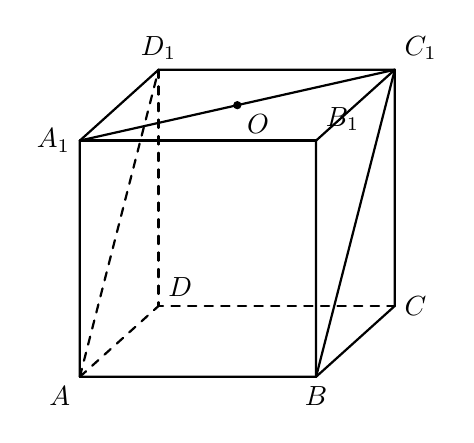
\begin{tikzpicture}[>=latex, line cap=round, line join=round, scale=1.0]
  % 顶点坐标
  \coordinate (A) at (0, 0);
  \coordinate (B) at (3, 0);
  \coordinate (C) at (4, 0.9);
  \coordinate (D) at (1, 0.9);
  
  \coordinate (A1) at (0, 3);
  \coordinate (B1) at (3, 3);
  \coordinate (C1) at (4, 3.9);
  \coordinate (D1) at (1, 3.9);
  
  \coordinate (O) at (2, 3.45);

  % 虚线棱与截面线
  \draw[dashed, thick] (D1) -- (D) -- (C);
  \draw[dashed, thick] (A) -- (D);
  \draw[dashed, thick] (A) -- (D1);

  % 实线棱与截面线
  \draw[thick] (A) -- (B) -- (C) -- (C1) -- (D1) -- (A1) -- cycle;
  \draw[thick] (B) -- (B1) -- (C1);
  \draw[thick] (A1) -- (B1);
  \draw[thick] (B) -- (C1);

  % 上底面对角线 A1C1 与中心 O
  \draw[thick] (A1) -- (C1);
  \fill (O) circle (1.5pt);
  \node[below right] at (O) {$O$};

  % 顶点标签
  \node[below left] at (A) {$A$};
  \node[below] at (B) {$B$};
  \node[right] at (C) {$C$};
  \node[above right] at (D) {$D$};
  \node[left] at (A1) {$A_1$};
  \node[above right] at (B1) {$B_1$};
  \node[above right] at (C1) {$C_1$};
  \node[above] at (D1) {$D_1$};
\end{tikzpicture}
\end{center}
\nopagebreak[4]
\begin{gkopts}(2)
\task A．$\dfrac{1}{2}$
\task B．$\dfrac{\sqrt{2}}{4}$
\task C．$\dfrac{\sqrt{2}}{2}$
\task D．$\dfrac{\sqrt{3}}{2}$
\end{gkopts}

\Needspace{4\baselineskip}
\textbf{解析}

以点 $D$ 为坐标原点，建立空间直角坐标系，使 $DA, DC, DD_1$ 分别为 $x, y, z$ 轴正方向．
\Needspace{5\baselineskip}
因为正方体棱长为 1，所以各顶点坐标为：
\nopagebreak[4]
\[
D(0, 0, 0), \quad A(1, 0, 0), \quad B(1, 1, 0), \quad C(0, 1, 0),
\]
\nopagebreak[4]
\[
A_1(1, 0, 1), \quad B_1(1, 1, 1), \quad C_1(0, 1, 1), \quad D_1(0, 0, 1).
\]
\Needspace{5\baselineskip}
点 $O$ 为上底面正方形 $A_1B_1C_1D_1$ 的中心，其坐标为：
\nopagebreak[4]
\[
O\left(\frac{1}{2}, \frac{1}{2}, 1\right).
\]
在平面 $ABC_1D_1$ 中，向量 $\vec{AB} = (0, 1, 0)$，$\vec{AD_1} = (-1, 0, 1)$．
\Needspace{5\baselineskip}
设平面 $ABC_1D_1$ 的一个法向量为 $\vec{n} = (x, y, z)$，则：
\nopagebreak[4]
\[
\begin{cases}
\vec{n} \cdot \vec{AB} = y = 0, \\
\vec{n} \cdot \vec{AD_1} = -x + z = 0 \implies x = z.
\end{cases}
\]
取 $x = z = 1$，得到法向量 $\vec{n} = (1, 0, 1)$．
\Needspace{5\baselineskip}
平面方程可写为：
\nopagebreak[4]
\[
1 \cdot (x - 1) + 0 \cdot (y - 0) + 1 \cdot (z - 0) = 0 \iff x + z - 1 = 0.
\]
\Needspace{5\baselineskip}
点 $O\left(\dfrac{1}{2}, \dfrac{1}{2}, 1\right)$ 到平面 $x + z - 1 = 0$ 的距离为：
\nopagebreak[4]
\[
d = \frac{\left|\frac{1}{2} + 1 - 1\right|}{\sqrt{1^2 + 0^2 + 1^2}} = \frac{\frac{1}{2}}{\sqrt{2}} = \frac{\sqrt{2}}{4}.
\]

故选 B．

\gkanswer{答案：B}

\end{answer}
\begin{answer}
\gksolhead{6}{}

\textbf{题目}：

设 $f_0(x) = \sin x, f_1(x) = f_0'(x), f_2(x) = f_1'(x), \dots, f_{n+1}(x) = f_n'(x), n \in \mathbf{N}$，则 $f_{2005}(x) =$\mbox{（　　）}

\begin{gkopts}(4)
\task A．$\sin x$
\task B．$-\sin x$
\task C．$\cos x$
\task D．$-\cos x$
\end{gkopts}

\Needspace{4\baselineskip}
\textbf{解析}

\Needspace{5\baselineskip}
函数的一阶至四阶导数分别为：
\nopagebreak[4]
\[
f_0(x) = \sin x,
\]
\nopagebreak[4]
\[
f_1(x) = f_0'(x) = \cos x,
\]
\nopagebreak[4]
\[
f_2(x) = f_1'(x) = -\sin x,
\]
\nopagebreak[4]
\[
f_3(x) = f_2'(x) = -\cos x,
\]
\nopagebreak[4]
\[
f_4(x) = f_3'(x) = \sin x = f_0(x).
\]
导函数的表达式具有周期性，周期为 4．
\Needspace{5\baselineskip}
因为 $2005 = 4 \times 501 + 1$，所以：
\nopagebreak[4]
\[
f_{2005}(x) = f_1(x) = \cos x.
\]

故选 C．

\gkanswer{答案：C}

\end{answer}
\begin{answer}
\gksolhead{7}{}

\textbf{题目}：

已知双曲线 $\dfrac{x^2}{a^2} - \dfrac{y^2}{b^2} = 1$ ($a > 0, b > 0$) 的右焦点为 $F$，右准线与一条渐近线交于点 $A$，$\triangle OAF$ 的面积为 $\dfrac{a^2}{2}$ ($O$ 为原点)，则两条渐近线的夹角为\mbox{（　　）}

\begin{gkopts}(4)
\task A．$30^\circ$
\task B．$45^\circ$
\task C．$60^\circ$
\task D．$90^\circ$
\end{gkopts}

\Needspace{4\baselineskip}
\textbf{解析}

双曲线 $\dfrac{x^2}{a^2} - \dfrac{y^2}{b^2} = 1$ 的右焦点为 $F(c, 0)$，右准线方程为 $x = \dfrac{a^2}{c}$．
其中一条渐近线方程为 $y = \dfrac{b}{a}x$．
\Needspace{5\baselineskip}
联立右准线与渐近线方程，得交点 $A$ 的坐标为：
\nopagebreak[4]
\[
x_A = \frac{a^2}{c}, \quad y_A = \frac{b}{a} \cdot \frac{a^2}{c} = \frac{ab}{c}.
\]
在 $\triangle OAF$ 中，底边 $OF = c$，高为点 $A$ 的纵坐标绝对值 $|y_A| = \dfrac{ab}{c}$．
\Needspace{5\baselineskip}
所以 $\triangle OAF$ 的面积为：
\nopagebreak[4]
\[
S_{\triangle OAF} = \frac{1}{2} \cdot c \cdot \frac{ab}{c} = \frac{1}{2}ab.
\]
\Needspace{5\baselineskip}
已知面积为 $\dfrac{a^2}{2}$，因此：
\nopagebreak[4]
\[
\frac{1}{2}ab = \frac{a^2}{2} \implies b = a.
\]
此时双曲线为等轴双曲线，两条渐近线方程分别为 $y = x$ 和 $y = -x$，斜率乘积为 $-1$，两条渐近线互相垂直，夹角为 $90^\circ$．

故选 D．

\gkanswer{答案：D}

\end{answer}
\begin{answer}
\gksolhead{8}{}

\textbf{题目}：

集合 $A = \left\{x \mid \dfrac{x - 1}{x + 1} < 0\right\}$，$B = \{x \mid |x - b| < a\}$，若“$a = 1$”是“$A \cap B \neq \varnothing$”的充分条件，则 $b$ 的取值范围是\mbox{（　　）}

\begin{gkopts}(2)
\task A．$-2 \leqslant b < 0$
\task B．$0 < b \leqslant 2$
\task C．$-3 < b < -1$
\task D．$-1 \leqslant b < 2$
\end{gkopts}

\Needspace{4\baselineskip}
\textbf{解析}

\Needspace{5\baselineskip}
解不等式化简集合 $A$：
\nopagebreak[4]
\[
\frac{x - 1}{x + 1} < 0 \iff (x - 1)(x + 1) < 0 \iff -1 < x < 1,
\]
即 $A = (-1, 1)$．
当 $a = 1$ 时，集合 $B = \{x \mid |x - b| < 1\} = (b - 1, b + 1)$．
“$a = 1$ 是 $A \cap B \neq \varnothing$ 的充分条件”等价于：当 $a = 1$ 时，必有 $A \cap B \neq \varnothing$．
\Needspace{5\baselineskip}
两开区间 $(-1, 1)$ 与 $(b - 1, b + 1)$ 有公共部分的充要条件为：
\nopagebreak[4]
\[
\begin{cases}
b - 1 < 1, \\
b + 1 > -1,
\end{cases}
\iff -2 < b < 2.
\]
即只要 $b \in (-2, 2)$，当 $a = 1$ 时必有 $A \cap B \neq \varnothing$．
四个选项中：
\begin{itemize}
\item 选项 A：$[-2, 0)$ 包含 $b = -2$，当 $b = -2$ 时 $B = (-3, -1)$，此时 $A \cap B = \varnothing$，充分性不成立；
\item 选项 B：$(0, 2]$ 包含 $b = 2$，当 $b = 2$ 时 $B = (1, 3)$，此时 $A \cap B = \varnothing$，充分性不成立；
\item 选项 C：$(-3, -1)$ 包含 $b \leqslant -2$ 的点，充分性不成立；
\item 选项 D：$[-1, 2) \subset (-2, 2)$，对任意 $b \in [-1, 2)$，均能保证 $A \cap B \neq \varnothing$ 成立．
\end{itemize}

故选 D．

\gkanswer{答案：D}

\end{answer}
\begin{answer}
\gksolhead{9}{}

\textbf{题目}：

4 位同学参加某种形式的竞赛，竞赛规则规定：每位同学必须从甲、乙两道题中任选一题作答，选甲题答对得 100 分，答错得 $-100$ 分；选乙题答对得 90 分，答错得 $-90$ 分．若 4 位同学的总分为 0，则这 4 位同学不同得分情况的种数是\mbox{（　　）}

\begin{gkopts}(4)
\task A．48
\task B．36
\task C．24
\task D．18
\end{gkopts}

\Needspace{4\baselineskip}
\textbf{解析}

每位同学的可能得分为：
\begin{itemize}
\item 选甲题答对得 100 分，答错得 $-100$ 分；
\item 选乙题答对得 90 分，答错得 $-90$ 分．
\end{itemize}
设 4 位同学中，选甲题答对的人数为 $k_1$，答错的人数为 $k_2$；选乙题答对的人数为 $m_1$，答错的人数为 $m_2$．
\Needspace{5\baselineskip}
各变量均为非负整数，且满足：
\nopagebreak[4]
\[
k_1 + k_2 + m_1 + m_2 = 4.
\]
\Needspace{5\baselineskip}
4 位同学的总分为：
\nopagebreak[4]
\[
100(k_1 - k_2) + 90(m_1 - m_2) = 0 \iff 10(k_1 - k_2) = -9(m_1 - m_2).
\]
因为 $\gcd(10, 9) = 1$，所以 $k_1 - k_2$ 必须是 9 的倍数．
\Needspace{5\baselineskip}
又因为 $0 \leqslant k_1, k_2 \leqslant 4$，所以 $|k_1 - k_2| \leqslant 4$，唯一的可能是：
\nopagebreak[4]
\[
k_1 - k_2 = 0 \implies k_1 = k_2, \quad m_1 - m_2 = 0 \implies m_1 = m_2.
\]
\Needspace{5\baselineskip}
代入总人数方程：
\nopagebreak[4]
\[
2k_1 + 2m_1 = 4 \implies k_1 + m_1 = 2.
\]
分三种情况讨论 4 位同学的得分组合：
1. $k_1 = 2, m_1 = 0$：
   4 人都选甲题，2 人得 100 分，2 人得 $-100$ 分．
\Needspace{5\baselineskip}
   分配给 4 位同学的方法数为：
\nopagebreak[4]
\[
\mathrm{C}_4^2 = 6 \text{ \text{种}}．
\]
2. $k_1 = 0, m_1 = 2$：
   4 人都选乙题，2 人得 90 分，2 人得 $-90$ 分．
\Needspace{5\baselineskip}
   分配给 4 位同学的方法数为：
\nopagebreak[4]
\[
\mathrm{C}_4^2 = 6 \text{ \text{种}}．
\]
3. $k_1 = 1, m_1 = 1$：
   4 位同学各得不同的分数：一人 100 分、一人 $-100$ 分、一人 90 分、一人 $-90$ 分．
\Needspace{5\baselineskip}
   分配给 4 位同学的方法数为：
\nopagebreak[4]
\[
\mathrm{A}_4^4 = 4! = 24 \text{ \text{种}}．
\]

\Needspace{5\baselineskip}
综合以上三种情况，4 位同学不同得分情况的种数共有：
\nopagebreak[4]
\[
6 + 6 + 24 = 36 \text{ \text{种}}．
\]

故选 B．

\gkanswer{答案：B}

\end{answer}
\begin{answer}
\gksolhead{10}{}

\textbf{题目}：

设 $P$ 是 $\triangle ABC$ 内任意一点，$S_{\triangle ABC}$ 表示 $\triangle ABC$ 的面积，$\lambda_1 = \dfrac{S_{\triangle PBC}}{S_{\triangle ABC}}, \lambda_2 = \dfrac{S_{\triangle PCA}}{S_{\triangle ABC}}, \lambda_3 = \dfrac{S_{\triangle PAB}}{S_{\triangle ABC}}$，定义 $f(P) = (\lambda_1, \lambda_2, \lambda_3)$，若 $G$ 是 $\triangle ABC$ 的重心，$f(Q) = \left(\dfrac{1}{2}, \dfrac{1}{3}, \dfrac{1}{6}\right)$，则\mbox{（　　）}

\begin{gkopts}(2)
\task A．点 $Q$ 在 $\triangle GAB$ 内
\task B．点 $Q$ 在 $\triangle GBC$ 内
\task C．点 $Q$ 在 $\triangle GCA$ 内
\task D．点 $Q$ 与点 $G$ 重合
\end{gkopts}

\Needspace{4\baselineskip}
\textbf{解析}

\Needspace{5\baselineskip}
根据题设，$(\lambda_1, \lambda_2, \lambda_3)$ 为点 $P$ 关于 $\triangle ABC$ 的面积坐标（重心坐标），满足：
\nopagebreak[4]
\[
\lambda_1 + \lambda_2 + \lambda_3 = 1 \quad (\lambda_1, \lambda_2, \lambda_3 > 0).
\]
\Needspace{5\baselineskip}
设三角形三个顶点为 $A, B, C$，其重心为 $G$．重心的面积坐标为：
\nopagebreak[4]
\[
f(G) = \left(\frac{1}{3}, \frac{1}{3}, \frac{1}{3}\right).
\]
\Needspace{5\baselineskip}
已知点 $Q$ 的面积坐标为：
\nopagebreak[4]
\[
f(Q) = \left(\frac{1}{2}, \frac{1}{3}, \frac{1}{6}\right).
\]

重心 $G$ 将 $\triangle ABC$ 分割为三个互不重叠的子三角形：$\triangle GAB, \triangle GBC, \triangle GCA$．
\Needspace{5\baselineskip}
在子三角形 $\triangle GAB$ 内部，任意点可由三个顶点 $A$、$B$、$G$ 的重心坐标凸组合表示：
\nopagebreak[4]
\[
Q = u A + v B + w G \quad (u > 0, v > 0, w > 0, u + v + w = 1).
\]
\Needspace{5\baselineskip}
因为顶点 $A$ 的面积坐标为 $(1, 0, 0)$，$B$ 为 $(0, 1, 0)$，$G$ 为 $\left(\dfrac{1}{3}, \dfrac{1}{3}, \dfrac{1}{3}\right)$，所以其线性组合为：
\nopagebreak[4]
\[
\begin{cases}
\lambda_1 = u + \dfrac{1}{3}w = \dfrac{1}{2}, \\
\lambda_2 = v + \dfrac{1}{3}w = \dfrac{1}{3}, \\
\lambda_3 = \dfrac{1}{3}w = \dfrac{1}{6}.
\end{cases}
\]
\Needspace{5\baselineskip}
由第三式直接解得：
\nopagebreak[4]
\[
w = 3 \times \frac{1}{6} = \frac{1}{2} > 0.
\]
\Needspace{5\baselineskip}
将其分别代入前两式：
\nopagebreak[4]
\[
u = \frac{1}{2} - \frac{1}{3} \times \frac{1}{2} = \frac{1}{2} - \frac{1}{6} = \frac{1}{3} > 0,
\]
\nopagebreak[4]
\[
v = \frac{1}{3} - \frac{1}{3} \times \frac{1}{2} = \frac{1}{3} - \frac{1}{6} = \frac{1}{6} > 0.
\]
系数满足 $u + v + w = \dfrac{1}{3} + \dfrac{1}{6} + \dfrac{1}{2} = 1$，且 $u > 0, v > 0, w > 0$ 均严格大于 0．
因此，点 $Q$ 落在以 $G, A, B$ 为顶点的三角形 $\triangle GAB$ 的内部．

故选 A．

\gkanswer{答案：A}

\end{answer}
\begin{answer}
\gksolhead{11}{}

\textbf{题目}：

一工厂生产了某种产品 16800 件，它们来自甲、乙、丙 3 条生产线，为检查这批产品的质量，决定采用分层抽样的方法进行抽样，已知甲、乙、丙三条生产线抽取的个体数组成一个等差数列，则乙生产线生产了\gkblank{}件产品．

\Needspace{4\baselineskip}
\textbf{解析}

设甲、乙、丙三条生产线抽取的个体数分别为 $n_1, n_2, n_3$．
\Needspace{5\baselineskip}
因为抽取的个体数组成一个等差数列，所以：
\nopagebreak[4]
\[
n_1 + n_3 = 2n_2.
\]
根据分层抽样的原理，各层抽取的样本数与该层总产品数成正比．
\Needspace{5\baselineskip}
设甲、乙、丙三条生产线生产的产品数分别为 $N_1, N_2, N_3$，则 $N_1, N_2, N_3$ 也成等差数列，即：
\nopagebreak[4]
\[
N_1 + N_3 = 2N_2.
\]
\Needspace{5\baselineskip}
又因为产品总数为 16800 件：
\nopagebreak[4]
\[
N_1 + N_2 + N_3 = 16800.
\]
\Needspace{5\baselineskip}
将 $N_1 + N_3 = 2N_2$ 代入得：
\nopagebreak[4]
\[
3N_2 = 16800 \implies N_2 = 5600.
\]
因此，乙生产线生产了 5600 件产品．

\gkanswer{答案：5600}

\end{answer}
\begin{answer}
\gksolhead{12}{}

\textbf{题目}：

在 $(1 + x) + (1 + x)^2 + \dots + (1 + x)^6$ 的展开式中，$x^2$ 项的系数是\gkblank{}．（用数字作答）

\Needspace{4\baselineskip}
\textbf{解析}

\Needspace{5\baselineskip}
根据二项式定理，$(1 + x)^k$ 的二项展开式为：
\nopagebreak[4]
\[
(1 + x)^k = \sum_{r=0}^k \mathrm{C}_k^r x^r.
\]
其中 $x^2$ 项的系数为 $\mathrm{C}_k^2$（当 $k \geqslant 2$ 时）．
\Needspace{5\baselineskip}
对于给定的多项式之和：
\nopagebreak[4]
\[
(1 + x) + (1 + x)^2 + (1 + x)^3 + (1 + x)^4 + (1 + x)^5 + (1 + x)^6,
\]
\Needspace{5\baselineskip}
各多项式中 $x^2$ 项系数之和为：
\nopagebreak[4]
\[
\sum_{k=2}^6 \mathrm{C}_k^2 = \mathrm{C}_2^2 + \mathrm{C}_3^2 + \mathrm{C}_4^2 + \mathrm{C}_5^2 + \mathrm{C}_6^2.
\]
\Needspace{5\baselineskip}
利用组合恒等式 $\mathrm{C}_n^m + \mathrm{C}_n^{m-1} = \mathrm{C}_{n+1}^m$ 进行累加：
\nopagebreak[4]
\[
\mathrm{C}_2^2 + \mathrm{C}_3^2 = \mathrm{C}_3^3 + \mathrm{C}_3^2 = \mathrm{C}_4^3,
\]
\nopagebreak[4]
\[
\mathrm{C}_4^3 + \mathrm{C}_4^2 = \mathrm{C}_5^3,
\]
\nopagebreak[4]
\[
\mathrm{C}_5^3 + \mathrm{C}_5^2 = \mathrm{C}_6^3,
\]
\nopagebreak[4]
\[
\mathrm{C}_6^3 + \mathrm{C}_6^2 = \mathrm{C}_7^3.
\]
\Needspace{5\baselineskip}
计算组合数：
\nopagebreak[4]
\[
\mathrm{C}_7^3 = \frac{7 \times 6 \times 5}{3 \times 2 \times 1} = 35.
\]
所以展开式中 $x^2$ 项的系数是 35．

\gkanswer{答案：35}

\end{answer}
\begin{answer}
\gksolhead{13}{}

\textbf{题目}：

已知直线 $ax + by + c = 0$ 与圆 $O: x^2 + y^2 = 1$ 相交于 $A$、$B$ 两点，且 $|AB| = \sqrt{3}$，则 $\vec{OA} \cdot \vec{OB} =$\gkblank{}．

\Needspace{4\baselineskip}
\textbf{解析}

圆 $O: x^2 + y^2 = 1$ 的圆心为坐标原点 $O(0, 0)$，半径 $R = 1$．
\Needspace{5\baselineskip}
因为点 $A, B$ 在圆 $O$ 上，所以：
\nopagebreak[4]
\[
|\vec{OA}| = 1, \quad |\vec{OB}| = 1.
\]
在 $\triangle OAB$ 中，三边长分别为 $OA = 1, OB = 1, AB = \sqrt{3}$．
\Needspace{5\baselineskip}
由余弦定理：
\nopagebreak[4]
\[
\cos \angle AOB = \frac{OA^2 + OB^2 - AB^2}{2 OA \cdot OB} = \frac{1^2 + 1^2 - (\sqrt{3})^2}{2 \times 1 \times 1} = \frac{2 - 3}{2} = -\frac{1}{2}.
\]
\Needspace{5\baselineskip}
根据向量数量积的定义：
\nopagebreak[4]
\[
\vec{OA} \cdot \vec{OB} = |\vec{OA}| |\vec{OB}| \cos \angle AOB = 1 \times 1 \times \left(-\frac{1}{2}\right) = -\frac{1}{2}.
\]

\gkanswer{答案：$-\dfrac{1}{2}$}

\end{answer}
\begin{answer}
\gksolhead{14}{}

\textbf{题目}：

设函数 $f(x)$ 的图象关于点 $(1, 2)$ 对称，且存在反函数 $f^{-1}(x)$，$f(4) = 0$，则 $f^{-1}(4) =$\gkblank{}．

\Needspace{4\baselineskip}
\textbf{解析}

函数 $f(x)$ 的图象关于点 $(1, 2)$ 中心对称．
若点 $(x, y)$ 在函数 $f(x)$ 的图象上，则其关于点 $(1, 2)$ 的对称点 $(2 \times 1 - x, 2 \times 2 - y) = (2 - x, 4 - y)$ 也在函数 $f(x)$ 的图象上．
已知 $f(4) = 0$，即点 $(4, 0)$ 在函数图象上．
\Needspace{5\baselineskip}
点 $(4, 0)$ 关于点 $(1, 2)$ 的对称点为：
\nopagebreak[4]
\[
(2 - 4, 4 - 0) = (-2, 4).
\]
\Needspace{5\baselineskip}
所以点 $(-2, 4)$ 必在函数 $f(x)$ 的图象上，即：
\nopagebreak[4]
\[
f(-2) = 4.
\]
\Needspace{5\baselineskip}
由反函数的定义，得：
\nopagebreak[4]
\[
f^{-1}(4) = -2.
\]

\gkanswer{答案：$-2$}

\end{answer}
\begin{answer}
\gksolhead{15}{}

\textbf{题目}：

设函数 $f(x)$ 的图象与直线 $x = a, x = b$ 及 $x$ 轴所围成图形的面积称为函数 $f(x)$ 在 $[a, b]$ 上的面积，已知函数 $y = \sin nx$ 在 $\left[0, \dfrac{\pi}{n}\right]$ 上的面积为 $\dfrac{2}{n}$ ($n \in \mathbf{N}^*$)．

(1) $y = \sin 3x$ 在 $\left[0, \dfrac{2\pi}{3}\right]$ 上的面积为\gkblank{}；

(2) $y = \sin(3x - \pi) + 1$ 在 $\left[\dfrac{\pi}{3}, \dfrac{4\pi}{3}\right]$ 上的面积为\gkblank{}．

\Needspace{4\baselineskip}
\textbf{解析}

\textbf{(1)}
函数 $y = \sin 3x$ 的最小正周期为 $T = \dfrac{2\pi}{3}$．
当 $x \in \left[0, \dfrac{\pi}{3}\right]$ 时，$\sin 3x \geqslant 0$；
当 $x \in \left[\dfrac{\pi}{3}, \dfrac{2\pi}{3}\right]$ 时，$\sin 3x \leqslant 0$．
根据题设，函数图象与 $x$ 轴所围成图形的面积取绝对值面积．
\Needspace{5\baselineskip}
在半周期 $\left[0, \dfrac{\pi}{3}\right]$ 上的面积为：
\nopagebreak[4]
\[
S_1 = \frac{2}{3}.
\]
\Needspace{5\baselineskip}
在半周期 $\left[\dfrac{\pi}{3}, \dfrac{2\pi}{3}\right]$ 上的面积由对称性同样为：
\nopagebreak[4]
\[
S_2 = \frac{2}{3}.
\]
\Needspace{5\baselineskip}
所以在区间 $\left[0, \dfrac{2\pi}{3}\right]$ 上的总面积为：
\nopagebreak[4]
\[
S = S_1 + S_2 = \frac{2}{3} + \frac{2}{3} = \frac{4}{3}.
\]

\textbf{(2)}
考察函数 $y = \sin(3x - \pi) + 1 = 1 - \sin 3x$．
\Needspace{5\baselineskip}
因为 $-1 \leqslant \sin 3x \leqslant 1$，所以在实数集上恒有：
\nopagebreak[4]
\[
y = 1 - \sin 3x \geqslant 0.
\]
\Needspace{5\baselineskip}
因此在区间 $\left[\dfrac{\pi}{3}, \dfrac{4\pi}{3}\right]$ 上，函数图象位于 $x$ 轴上方（除在极值点处与 $x$ 轴相切外），所围成图形的面积即为该函数的定积分：
\nopagebreak[4]
\[
S = \int_{\pi/3}^{4\pi/3} (1 - \sin 3x)\,\mathrm{d}x.
\]
\Needspace{5\baselineskip}
求原函数并计算积分值：
\nopagebreak[4]
\[
S = \left[x + \frac{1}{3}\cos 3x\right]_{\pi/3}^{4\pi/3} = \left(\frac{4\pi}{3} - \frac{\pi}{3}\right) + \frac{1}{3}\left[\cos(4\pi) - \cos(\pi)\right].
\]
\Needspace{5\baselineskip}
计算各项：
\nopagebreak[4]
\[
\frac{4\pi}{3} - \frac{\pi}{3} = \pi,
\]
\nopagebreak[4]
\[
\cos(4\pi) - \cos(\pi) = 1 - (-1) = 2.
\]
\Needspace{5\baselineskip}
代入得：
\nopagebreak[4]
\[
S = \pi + \frac{2}{3}.
\]

\gkanswer{答案（1）：$\dfrac{4}{3}$。}

\gkanswer{答案（2）：$\pi + \dfrac{2}{3}$。}

\end{answer}
\begin{answer}
\gksolhead{16}{}

\textbf{题目}：

已知在 $\triangle ABC$ 中，$\sin A(\sin B + \cos B) - \sin C = 0, \sin B + \cos 2C = 0$，求角 $A, B, C$ 的大小．

\Needspace{4\baselineskip}
\textbf{解析}

\Needspace{5\baselineskip}
在 $\triangle ABC$ 中，因为 $A + B + C = \pi$，所以：
\nopagebreak[4]
\[
\sin C = \sin[\pi - (A + B)] = \sin(A + B) = \sin A\cos B + \cos A\sin B.
\]
\Needspace{5\baselineskip}
将其代入已知第一个方程：
\nopagebreak[4]
\[
\sin A(\sin B + \cos B) - (\sin A\cos B + \cos A\sin B) = 0.
\]
\Needspace{5\baselineskip}
展开消去同类项：
\nopagebreak[4]
\[
\sin A\sin B + \sin A\cos B - \sin A\cos B - \cos A\sin B = 0,
\]
\nopagebreak[4]
\[
\sin B(\sin A - \cos A) = 0.
\]
因为在三角形中 $B \in (0, \pi)$，正弦值严格为正，即 $\sin B > 0$．
\Needspace{5\baselineskip}
所以必须有：
\nopagebreak[4]
\[
\sin A - \cos A = 0 \implies \tan A = 1.
\]
\Needspace{5\baselineskip}
又因为 $A \in (0, \pi)$，解得：
\nopagebreak[4]
\[
A = \frac{\pi}{4}.
\]
\Needspace{5\baselineskip}
将 $A = \dfrac{\pi}{4}$ 代入三角形内角和定理：
\nopagebreak[4]
\[
B + C = \pi - \frac{\pi}{4} = \frac{3\pi}{4} \implies B = \frac{3\pi}{4} - C.
\]
\Needspace{5\baselineskip}
再结合第二个已知方程 $\sin B + \cos 2C = 0$：
\nopagebreak[4]
\[
\sin B = -\cos 2C = \sin\left(2C - \frac{\pi}{2}\right).
\]
\Needspace{5\baselineskip}
将 $B = \dfrac{3\pi}{4} - C$ 代入：
\nopagebreak[4]
\[
\sin\left(\frac{3\pi}{4} - C\right) = \sin\left(2C - \frac{\pi}{2}\right).
\]
因为 $C \in \left(0, \dfrac{3\pi}{4}\right)$，所以角满足以下两种情况：
\Needspace{5\baselineskip}
1. 若 $\dfrac{3\pi}{4} - C = 2C - \dfrac{\pi}{2}$，则：
\nopagebreak[4]
\[
3C = \frac{5\pi}{4} \implies C = \frac{5\pi}{12}.
\]
\Needspace{5\baselineskip}
   代入求 $B$：
\nopagebreak[4]
\[
B = \frac{3\pi}{4} - \frac{5\pi}{12} = \frac{\pi}{3}.
\]
   此时检验：$\sin B = \sin \dfrac{\pi}{3} = \dfrac{\sqrt{3}}{2}$，$\cos 2C = \cos \dfrac{5\pi}{6} = -\dfrac{\sqrt{3}}{2}$，两者之和为 0，符合题意．
\Needspace{5\baselineskip}
2. 若 $\left(\dfrac{3\pi}{4} - C\right) + \left(2C - \dfrac{\pi}{2}\right) = \pi$，则：
\nopagebreak[4]
\[
C + \frac{\pi}{4} = \pi \implies C = \frac{3\pi}{4}.
\]
   此时 $B = \dfrac{3\pi}{4} - \dfrac{3\pi}{4} = 0$，不符合三角形内角要求，舍去．

\Needspace{5\baselineskip}
综上所述，三个角的大小分别为：
\nopagebreak[4]
\[
A = \frac{\pi}{4}, \quad B = \frac{\pi}{3}, \quad C = \frac{5\pi}{12}.
\]

\gkanswer{答案：$A = \dfrac{\pi}{4}, B = \dfrac{\pi}{3}, C = \dfrac{5\pi}{12}$}

\end{answer}
\begin{answer}
\gksolhead{17}{}

\textbf{题目}：

如图 1，已知 $ABCD$ 是上、下底边长分别为 2 和 6，高为 $\sqrt{3}$ 的等腰梯形，将它沿对称轴 $OO_1$ 折成直二面角，如图 2．
\nopagebreak[4]
\begin{center}% 2005 年湖南卷理科第 17 题配图：等腰梯形折成直二面角（图 1 与图 2）
\begin{tikzpicture}[>=latex, line cap=round, line join=round, scale=0.9]
  % ----------------- 图 1 -----------------
  \begin{scope}[shift={(0, 0)}]
    \coordinate (O) at (0, 0);
    \coordinate (A) at (-2.4, 0);
    \coordinate (B) at (2.4, 0);
    \coordinate (O1) at (0, 1.6);
    \coordinate (D) at (-0.8, 1.6);
    \coordinate (C) at (0.8, 1.6);

    \draw[thick] (A) -- (B) -- (C) -- (D) -- cycle;
    \draw[thick] (O) -- (O1);

    \node[below left] at (A) {$A$};
    \node[below right] at (B) {$B$};
    \node[below] at (O) {$O$};
    \node[above] at (O1) {$O_1$};
    \node[above left] at (D) {$D$};
    \node[above right] at (C) {$C$};

    \node[below] at (0, -0.6) {图 1};
  \end{scope}

  % ----------------- 图 2 -----------------
  \begin{scope}[shift={(5.5, 0)}]
    \coordinate (O) at (0, 0);
    \coordinate (O1) at (0, 2.0);
    \coordinate (B) at (2.4, 0);
    \coordinate (C) at (0.8, 2.0);
    \coordinate (A) at (-0.7, -1.0);
    \coordinate (D) at (-0.4, 1.7);

    % 虚线：转折轴 OO1
    \draw[dashed, thick] (O) -- (O1);

    % 实线边与辅助线（AC 与 BO1）
    \draw[thick] (O) -- (B) -- (C) -- (O1);
    \draw[thick] (O) -- (A) -- (D) -- (O1);
    \draw[thick] (B) -- (O1);
    \draw[thick] (A) -- (C);

    % 顶点标签
    \node[below right] at (O) {$O$};
    \node[above] at (O1) {$O_1$};
    \node[right] at (B) {$B$};
    \node[above right] at (C) {$C$};
    \node[below left] at (A) {$A$};
    \node[left] at (D) {$D$};

    \node[below] at (0.8, -1.2) {图 2};
  \end{scope}
\end{tikzpicture}
\end{center}
\nopagebreak[4]
(1) 证明：$AC \perp BO_1$；

(2) 求二面角 $O - AC - O_1$ 的大小．

\Needspace{4\baselineskip}
\textbf{解析}

\textbf{(1)}
在等腰梯形 $ABCD$ 中，$AD = BC$，$AB \parallel CD$，$OO_1$ 是对称轴．
折起前在图 1 中：$OO_1 \perp AB$，$OO_1 \perp CD$，$OA = OB = 3$，$O_1D = O_1C = 1$，$OO_1 = \sqrt{3}$．
将梯形沿 $OO_1$ 折成直二面角，则平面 $AOO_1D \perp$ 平面 $BOO_1C$．
以 $O$ 为原点，建立空间直角坐标系：
取射线 $OA$ 为 $x$ 轴正方向，射线 $OB$ 为 $y$ 轴正方向，射线 $OO_1$ 为 $z$ 轴正方向．
因为二面角为直二面角，所以 $x$ 轴、$y$ 轴、$z$ 轴两两垂直．
\Needspace{5\baselineskip}
各顶点的空间直角坐标为：
\nopagebreak[4]
\[
O(0, 0, 0), \quad A(3, 0, 0), \quad B(0, 3, 0),
\]
\nopagebreak[4]
\[
O_1(0, 0, \sqrt{3}), \quad D(1, 0, \sqrt{3}), \quad C(0, 1, \sqrt{3}).
\]
\Needspace{5\baselineskip}
计算向量 $\vec{AC}$ 与 $\vec{BO_1}$ 的坐标：
\nopagebreak[4]
\[
\vec{AC} = (0 - 3, 1 - 0, \sqrt{3} - 0) = (-3, 1, \sqrt{3}),
\]
\nopagebreak[4]
\[
\vec{BO_1} = (0 - 0, 0 - 3, \sqrt{3} - 0) = (0, -3, \sqrt{3}).
\]
\Needspace{5\baselineskip}
计算两向量的数量积：
\nopagebreak[4]
\[
\vec{AC} \cdot \vec{BO_1} = (-3) \times 0 + 1 \times (-3) + \sqrt{3} \times \sqrt{3} = 0 - 3 + 3 = 0.
\]
所以 $\vec{AC} \perp \vec{BO_1}$，即 $AC \perp BO_1$．

\textbf{(2)}
求二面角 $O - AC - O_1$ 的大小：
在平面 $OAC$ 中，$\vec{OA} = (3, 0, 0)$，$\vec{OC} = (0, 1, \sqrt{3})$．
\Needspace{5\baselineskip}
设平面 $OAC$ 的一个法向量为 $\vec{n}_1 = (x, y, z)$，则：
\nopagebreak[4]
\[
\begin{cases}
\vec{n}_1 \cdot \vec{OA} = 3x = 0 \implies x = 0, \\
\vec{n}_1 \cdot \vec{OC} = y + \sqrt{3}z = 0 \implies y = -\sqrt{3}z.
\end{cases}
\]
取 $z = 1$，得 $\vec{n}_1 = (0, -\sqrt{3}, 1)$．

在平面 $O_1AC$ 中，$\vec{O_1C} = (0, 1, 0)$，$\vec{O_1A} = (3, 0, -\sqrt{3})$．
\Needspace{5\baselineskip}
设平面 $O_1AC$ 的一个法向量为 $\vec{n}_2 = (x, y, z)$，则：
\nopagebreak[4]
\[
\begin{cases}
\vec{n}_2 \cdot \vec{O_1C} = y = 0, \\
\vec{n}_2 \cdot \vec{O_1A} = 3x - \sqrt{3}z = 0 \implies z = \sqrt{3}x.
\end{cases}
\]
取 $x = 1$，得 $\vec{n}_2 = (1, 0, \sqrt{3})$．

\Needspace{5\baselineskip}
设二面角 $O - AC - O_1$ 的平面角大小为 $\theta$（$0 \leqslant \theta \leqslant \pi$），则：
\nopagebreak[4]
\[
\cos\theta = \frac{|\vec{n}_1 \cdot \vec{n}_2|}{|\vec{n}_1| |\vec{n}_2|} = \frac{|0 \times 1 + (-\sqrt{3}) \times 0 + 1 \times \sqrt{3}|}{\sqrt{0^2 + (-\sqrt{3})^2 + 1^2} \sqrt{1^2 + 0^2 + (\sqrt{3})^2}} = \frac{\sqrt{3}}{\sqrt{4}\sqrt{4}} = \frac{\sqrt{3}}{4}.
\]
所以二面角 $O - AC - O_1$ 的大小为 $\arccos \dfrac{\sqrt{3}}{4}$．

\gkanswer{答案（1）：证明见解析。}

\gkanswer{答案（2）：$\arccos \dfrac{\sqrt{3}}{4}$。}

\end{answer}
\begin{answer}
\gksolhead{18}{}

\textbf{题目}：

某城市有甲、乙、丙 3 个旅游景点，一位客人游览这三个景点的概率分别是 $0.4, 0.5, 0.6$，且客人是否游览哪个景点互不影响，设 $\xi$ 表示客人离开该城市时游览的景点数与没有游览的景点数之差的绝对值．

(1) 求 $\xi$ 的分布及数学期望；

(2) 记“函数 $f(x) = x^2 - 3\xi x + 1$ 在区间 $[2, +\infty)$ 上单调递增”为事件 $A$，求事件 $A$ 的概率．

\Needspace{4\baselineskip}
\textbf{解析}

\textbf{(1)}
设该客人游览的景点数为 $X$，则没有游览的景点数为 $3 - X$．
\Needspace{5\baselineskip}
随机变量 $\xi$ 表示两者之差的绝对值，即：
\nopagebreak[4]
\[
\xi = |X - (3 - X)| = |2X - 3|.
\]
\Needspace{5\baselineskip}
因为该客人游览各个景点的事件相互独立，设游览甲、乙、丙三个景点的事件分别为 $A_1, A_2, A_3$，其概率分别为：
\nopagebreak[4]
\[
P(A_1) = 0.4, \quad P(A_2) = 0.5, \quad P(A_3) = 0.6.
\]
$X$ 的可能取值为 $0, 1, 2, 3$：
\begin{itemize}
\item 当 $X = 0$ 时，$\xi = |0 - 3| = 3$；
\item 当 $X = 1$ 时，$\xi = |2 - 3| = 1$；
\item 当 $X = 2$ 时，$\xi = |4 - 3| = 1$；
\item 当 $X = 3$ 时，$\xi = |6 - 3| = 3$．
\end{itemize}

\Needspace{5\baselineskip}
计算各个概率：
\nopagebreak[4]
\[
P(X = 0) = (1 - 0.4)(1 - 0.5)(1 - 0.6) = 0.6 \times 0.5 \times 0.4 = 0.12,
\]
\nopagebreak[4]
\[
P(X = 3) = 0.4 \times 0.5 \times 0.6 = 0.12.
\]
\Needspace{5\baselineskip}
由此可得 $\xi = 3$ 的概率为：
\nopagebreak[4]
\[
P(\xi = 3) = P(X = 0) + P(X = 3) = 0.12 + 0.12 = 0.24.
\]
\Needspace{5\baselineskip}
因为 $\xi$ 的取值只有 1 和 3，所以 $\xi = 1$ 的概率为：
\nopagebreak[4]
\[
P(\xi = 1) = 1 - P(\xi = 3) = 1 - 0.24 = 0.76.
\]
\Needspace{5\baselineskip}
故 $\xi$ 的分布列为：
\nopagebreak[4]
\[
P(\xi = 1) = 0.76, \quad P(\xi = 3) = 0.24.
\]
\Needspace{5\baselineskip}
数学期望为：
\nopagebreak[4]
\[
\mathbf{E}\xi = 1 \times 0.76 + 3 \times 0.24 = 0.76 + 0.72 = 1.48.
\]

\textbf{(2)}
\Needspace{5\baselineskip}
二次函数 $f(x) = x^2 - 3\xi x + 1$ 的图象开口向上，其对称轴为：
\nopagebreak[4]
\[
x = \frac{3\xi}{2}.
\]
\Needspace{5\baselineskip}
函数在区间 $[2, +\infty)$ 上单调递增，当且仅当对称轴位于区间左端点的左侧或端点处，即：
\nopagebreak[4]
\[
\frac{3\xi}{2} \leqslant 2 \iff \xi \leqslant \frac{4}{3}.
\]
因为 $\xi$ 的可能取值为 1 和 3：
\begin{itemize}
\item 当 $\xi = 1$ 时，$\dfrac{3}{2} \leqslant 2$ 成立；
\item 当 $\xi = 3$ 时，$\dfrac{9}{2} > 2$ 不成立．
\end{itemize}

因此，事件 $A$ 发生等价于 $\xi = 1$．
\Needspace{5\baselineskip}
故事件 $A$ 的概率为：
\nopagebreak[4]
\[
P(A) = P(\xi = 1) = 0.76.
\]

\gkanswer{答案（1）：$\xi$ 的分布列为 $P(\xi=1)=0.76, P(\xi=3)=0.24$；数学期望 $\mathbf{E}\xi = 1.48$。}

\gkanswer{答案（2）：$0.76$。}

\end{answer}
\begin{answer}
\gksolhead{19}{}

\textbf{题目}：

已知椭圆 $C: \dfrac{x^2}{a^2} + \dfrac{y^2}{b^2} = 1$ ($a > b > 0$) 的左、右焦点为 $F_1, F_2$，离心率为 $e$．直线 $l: y = ex + a$ 与 $x$ 轴、$y$ 轴分别交于点 $A, B$，$M$ 是直线 $l$ 与椭圆 $C$ 的一个公共点，$P$ 是点 $F_1$ 关于直线 $l$ 的对称点，设 $\vec{AM} = \lambda\vec{AB}$．

(1) 证明：$\lambda = 1 - e^2$；

(2) 确定 $\lambda$ 的值，使得 $\triangle PF_1F_2$ 是等腰三角形．

\Needspace{4\baselineskip}
\textbf{解析}

\textbf{(1)}
直线 $l$ 的方程为 $y = ex + a$．
令 $y = 0$，得点 $A$ 的坐标为 $A\left(-\dfrac{a}{e}, 0\right)$；
令 $x = 0$，得点 $B$ 的坐标为 $B(0, a)$．
向量 $\vec{AB} = \left(\dfrac{a}{e}, a\right)$．
\Needspace{5\baselineskip}
由已知 $\vec{AM} = \lambda \vec{AB}$，可得点 $M$ 的坐标为：
\nopagebreak[4]
\[
M = A + \lambda \vec{AB} = \left(-\frac{a}{e} + \lambda \frac{a}{e}, \lambda a\right) = \left(\frac{(\lambda - 1)a}{e}, \lambda a\right).
\]
\Needspace{5\baselineskip}
因为点 $M$ 在椭圆 $C: \dfrac{x^2}{a^2} + \dfrac{y^2}{b^2} = 1$ 上，将其坐标代入椭圆方程：
\nopagebreak[4]
\[
\frac{\left[\frac{(\lambda - 1)a}{e}\right]^2}{a^2} + \frac{(\lambda a)^2}{b^2} = 1 \iff \frac{(\lambda - 1)^2}{e^2} + \frac{\lambda^2 a^2}{b^2} = 1.
\]
\Needspace{5\baselineskip}
由于 $b^2 = a^2(1 - e^2)$，代入上式得：
\nopagebreak[4]
\[
\frac{(\lambda - 1)^2}{e^2} + \frac{\lambda^2}{1 - e^2} = 1.
\]
\Needspace{5\baselineskip}
两边同乘以 $e^2(1 - e^2)$：
\nopagebreak[4]
\[
(1 - e^2)(\lambda - 1)^2 + e^2\lambda^2 = e^2(1 - e^2).
\]
\Needspace{5\baselineskip}
展开左边并整理：
\nopagebreak[4]
\[
(1 - e^2)(\lambda^2 - 2\lambda + 1) + e^2\lambda^2 = \lambda^2 - 2(1 - e^2)\lambda + (1 - e^2).
\]
\Needspace{5\baselineskip}
将右边 $e^2(1 - e^2)$ 移到左边：
\nopagebreak[4]
\[
\lambda^2 - 2(1 - e^2)\lambda + (1 - e^2) - e^2(1 - e^2) = 0,
\]
\nopagebreak[4]
\[
\lambda^2 - 2(1 - e^2)\lambda + (1 - e^2)^2 = 0.
\]
\Needspace{5\baselineskip}
配方得：
\nopagebreak[4]
\[
[\lambda - (1 - e^2)]^2 = 0.
\]
\Needspace{5\baselineskip}
所以方程有唯一解：
\nopagebreak[4]
\[
\lambda = 1 - e^2.
\]

\textbf{(2)}
焦点坐标为 $F_1(-c, 0), F_2(c, 0)$，半焦距 $c = ea$．
直线 $l$ 的一般式方程为 $ex - y + a = 0$．
\Needspace{5\baselineskip}
点 $F_1(-c, 0) = (-ea, 0)$ 到直线 $l$ 的距离为：
\nopagebreak[4]
\[
d = \frac{|e(-ea) - 0 + a|}{\sqrt{e^2 + 1}} = \frac{a(1 - e^2)}{\sqrt{1 + e^2}}.
\]
\Needspace{5\baselineskip}
因为点 $P$ 是点 $F_1$ 关于直线 $l$ 的对称点，所以：
\nopagebreak[4]
\[
|PF_1| = 2d = \frac{2a(1 - e^2)}{\sqrt{1 + e^2}}.
\]
\Needspace{5\baselineskip}
根据椭圆的光学性质，直线 $l$ 是椭圆在点 $M$ 处的切线，点 $F_1$ 关于切线 $l$ 的对称点 $P$ 必落在射线 $F_2M$ 的延长线上，且有：
\nopagebreak[4]
\[
|PF_2| = |PM| + |MF_2| = |MF_1| + |MF_2| = 2a.
\]
\Needspace{5\baselineskip}
两焦点之间的距离为：
\nopagebreak[4]
\[
|F_1F_2| = 2c = 2ea.
\]
\Needspace{5\baselineskip}
在 $\triangle PF_1F_2$ 中，三边长分别为：
\nopagebreak[4]
\[
|PF_2| = 2a, \quad |F_1F_2| = 2ea, \quad |PF_1| = \frac{2a(1 - e^2)}{\sqrt{1 + e^2}}.
\]
\Needspace{5\baselineskip}
因为离心率 $0 < e < 1$，所以：
\nopagebreak[4]
\[
|F_1F_2| = 2ea < 2a = |PF_2|,
\]
\nopagebreak[4]
\[
|PF_1| = \frac{2a(1 - e^2)}{\sqrt{1 + e^2}} < 2a = |PF_2|.
\]
\Needspace{5\baselineskip}
要使 $\triangle PF_1F_2$ 为等腰三角形，只能是两条较短边相等，即：
\nopagebreak[4]
\[
|PF_1| = |F_1F_2|.
\]
\Needspace{5\baselineskip}
代入边长得：
\nopagebreak[4]
\[
\frac{2a(1 - e^2)}{\sqrt{1 + e^2}} = 2ea \iff \frac{1 - e^2}{\sqrt{1 + e^2}} = e.
\]
\Needspace{5\baselineskip}
两边平方并整理：
\nopagebreak[4]
\[
\frac{(1 - e^2)^2}{1 + e^2} = e^2 \iff 1 - 2e^2 + e^4 = e^2 + e^4,
\]
\nopagebreak[4]
\[
1 - 3e^2 = 0 \implies e^2 = \frac{1}{3}.
\]
因为 $0 < e < 1$，所以 $e = \dfrac{\sqrt{3}}{3}$．
\Needspace{5\baselineskip}
此时：
\nopagebreak[4]
\[
\lambda = 1 - e^2 = 1 - \frac{1}{3} = \frac{2}{3}.
\]
经检验，此时三边长满足两边之和大于第三边，点 $P, F_1, F_2$ 不共线，能构成等腰三角形．
故使得 $\triangle PF_1F_2$ 是等腰三角形的 $\lambda$ 的值为 $\dfrac{2}{3}$．

\gkanswer{答案（1）：证明见解析。}

\gkanswer{答案（2）：$\dfrac{2}{3}$。}

\end{answer}
\begin{answer}
\gksolhead{20}{}

\textbf{题目}：

自然状态下的鱼类是一种可再生资源，为持续利用这一资源，需从宏观上考察其再生能力及捕捞强度对鱼群总量的影响．用 $x_n$ 表示某鱼群在第 $n$ 年年初的总量，$n \in \mathbf{N}^*$，且 $x_1 > 0$．不考虑其它因素，设在第 $n$ 年内鱼群的繁殖量及捕捞量都与 $x_n$ 成正比，死亡量与 $x_n^2$ 成正比，这些比例系数依次为正常数 $a, b, c$．

(1) 求 $x_{n+1}$ 与 $x_n$ 的关系式；

(2) 猜测：当且仅当 $x_1, a, b, c$ 满足什么条件时，每年年初鱼群的总量保持不变？（不要求证明）

(3) 设 $a = 2, c = 1$（原卷印作 $b = 1$），为保证对任意 $x_1 \in (0, 2)$，都有 $x_n > 0, n \in \mathbf{N}^*$，则捕捞强度 $b$ 的最大允许值是多少？证明你的结论．

\Needspace{4\baselineskip}
\textbf{解析}

\textbf{(1)}
根据题设，第 $n$ 年内：
\begin{itemize}
\item 繁殖量与年初总量 $x_n$ 成正比，比例系数为 $a$，故繁殖量为 $ax_n$；
\item 捕捞量与年初总量 $x_n$ 成正比，比例系数为 $b$，故捕捞量为 $bx_n$；
\item 死亡量与年初总量平方 $x_n^2$ 成正比，比例系数为 $c$，故死亡量为 $cx_n^2$．
\end{itemize}

\Needspace{5\baselineskip}
第 $n+1$ 年年初的总量等于第 $n$ 年年初的总量加上该年内的繁殖量，减去捕捞量和死亡量：
\nopagebreak[4]
\[
x_{n+1} = x_n + ax_n - bx_n - cx_n^2 = (1 + a - b)x_n - cx_n^2.
\]

\textbf{(2)}
若每年年初鱼群的总量保持不变，即对一切 $n \in \mathbf{N}^*$，均有 $x_{n+1} = x_n = x_1$．
\Needspace{5\baselineskip}
将此条件代入递推关系式：
\nopagebreak[4]
\[
x_1 = (1 + a - b)x_1 - cx_1^2.
\]
\Needspace{5\baselineskip}
因为 $x_1 > 0$，两边同除以 $x_1$：
\nopagebreak[4]
\[
1 = 1 + a - b - cx_1 \implies cx_1 = a - b \implies x_1 = \frac{a - b}{c}.
\]
因为 $c > 0$ 且 $x_1 > 0$，所以必须有 $a > b$．
因此，当且仅当 $a > b$ 且 $x_1 = \dfrac{a - b}{c}$ 时，每年年初鱼群的总量保持不变．

\textbf{(3)}
\Needspace{5\baselineskip}
将参数 $a = 2, c = 1$ 代入递推式：
\nopagebreak[4]
\[
x_{n+1} = (1 + 2 - b)x_n - x_n^2 = (3 - b)x_n - x_n^2.
\]
构造函数 $f(x) = (3 - b)x - x^2$（$x > 0$）．
要保证对任意 $x_1 \in (0, 2)$，都有 $x_n > 0$（$n \in \mathbf{N}^*$）：
当 $n = 2$ 时，$x_2 = f(x_1) = x_1(3 - b - x_1) > 0$ 必须对任意 $x_1 \in (0, 2)$ 恒成立．
\Needspace{5\baselineskip}
因为 $x_1 > 0$，所以必有：
\nopagebreak[4]
\[
3 - b - x_1 > 0 \iff x_1 < 3 - b \quad (\forall x_1 \in (0, 2)).
\]
从而有 $3 - b \geqslant 2 \implies b \leqslant 1$．
下面证明当 $b = 1$ 时，对任意 $x_1 \in (0, 2)$，都有 $x_n > 0$ 对所有 $n \in \mathbf{N}^*$ 成立：
\Needspace{5\baselineskip}
当 $b = 1$ 时，递推关系式为：
\nopagebreak[4]
\[
x_{n+1} = 2x_n - x_n^2 = -(x_n - 1)^2 + 1.
\]
利用数学归纳法证明命题：对任意 $n \geqslant 2$，均有 $0 < x_n \leqslant 1$．
1. 当 $n = 2$ 时，因为 $x_1 \in (0, 2)$，所以 $x_1 - 1 \in (-1, 1)$，
   从而 $(x_1 - 1)^2 \in [0, 1)$，
   所以 $x_2 = 1 - (x_1 - 1)^2 \in (0, 1]$，即 $0 < x_2 \leqslant 1$ 成立；
2. 假设当 $n = k$（$k \geqslant 2$）时，命题成立，即 $0 < x_k \leqslant 1$．
\Needspace{5\baselineskip}
   则当 $n = k + 1$ 时：
\nopagebreak[4]
\[
x_{k+1} = 2x_k - x_k^2 = x_k(2 - x_k).
\]
   因为 $0 < x_k \leqslant 1$，所以 $1 \leqslant 2 - x_k < 2$，
   因此 $x_{k+1} = x_k(2 - x_k) > 0$．
   又 $x_{k+1} = 1 - (x_k - 1)^2 \leqslant 1$，所以 $0 < x_{k+1} \leqslant 1$ 同样成立．
由数学归纳法可知，对任意 $n \in \mathbf{N}^*$，恒有 $x_n > 0$．
综上所述，捕捞强度 $b$ 的最大允许值为 1．

\gkanswer{答案（1）：$x_{n+1} = (1 + a - b)x_n - cx_n^2$。}

\gkanswer{答案（2）：$a > b$ 且 $x_1 = \dfrac{a - b}{c}$。}

\gkanswer{答案（3）：捕捞强度 $b$ 的最大允许值是 $1$。}

\end{answer}
\begin{answer}
\gksolhead{21}{}

\textbf{题目}：

已知函数 $f(x) = \ln x, g(x) = \dfrac{1}{2}ax^2 + bx, a \neq 0$．

(1) 若 $b = 2$，且 $h(x) = f(x) - g(x)$ 存在单调递减区间，求 $a$ 的取值范围；

(2) 设函数 $f(x)$ 的图象 $C_1$ 与函数 $g(x)$ 图象 $C_2$ 交于点 $P$、$Q$，过线段 $PQ$ 的中点作 $x$ 轴的垂线分别交 $C_1, C_2$ 于点 $M$、$N$，证明 $C_1$ 在点 $M$ 处的切线与 $C_2$ 在点 $N$ 处的切线不平行．

\Needspace{4\baselineskip}
\textbf{解析}

\textbf{(1)}
\Needspace{5\baselineskip}
当 $b = 2$ 时，$g(x) = \dfrac{1}{2}ax^2 + 2x$，因此：
\nopagebreak[4]
\[
h(x) = f(x) - g(x) = \ln x - \frac{1}{2}ax^2 - 2x \quad (x > 0).
\]
\Needspace{5\baselineskip}
对其求导：
\nopagebreak[4]
\[
h'(x) = \frac{1}{x} - ax - 2 = \frac{-ax^2 - 2x + 1}{x}.
\]
因为定义域为 $(0, +\infty)$，分母 $x > 0$，$h(x)$ 存在单调递减区间等价于：
\Needspace{5\baselineskip}
不等式 $h'(x) < 0$ 在 $(0, +\infty)$ 上有解，即存在 $x \in (0, +\infty)$ 使得：
\nopagebreak[4]
\[
-ax^2 - 2x + 1 < 0 \iff ax^2 > 1 - 2x.
\]
分情况讨论：
\begin{itemize}
\item 若 $a > 0$：当 $x \to +\infty$ 时，$ax^2 \to +\infty$，而 $1 - 2x \to -\infty$，因此对充分大的 $x$，恒有 $ax^2 > 1 - 2x$ 成立，$h(x)$ 必然存在单调递减区间；
\item 若 $a < 0$：二次函数 $y = -ax^2 - 2x + 1$ 的二次项系数 $-a > 0$，图象开口向上，且当 $x = 0$ 时值为 $1 > 0$．
\end{itemize}
  其对称轴为 $x = \dfrac{2}{2(-a)} = -\dfrac{1}{a} > 0$．
\Needspace{5\baselineskip}
  要使其在 $(0, +\infty)$ 内有函数值小于 0，必须且只需判别式大于 0：
\nopagebreak[4]
\[
\Delta = (-2)^2 - 4(-a)(1) = 4 + 4a > 0 \iff a > -1.
\]
  此时方程有两个正根，在两根之间恒有 $-ax^2 - 2x + 1 < 0$．

综合上述讨论，实数 $a$ 的取值范围是 $(-1, 0) \cup (0, +\infty)$．

\textbf{(2)}
设曲线 $C_1$ 与 $C_2$ 的交点分别为 $P(x_1, y_1), Q(x_2, y_2)$，不妨设 $0 < x_1 < x_2$．
\Needspace{5\baselineskip}
因为 $P, Q$ 是交点，所以其坐标同时满足两曲线方程：
\nopagebreak[4]
\[
\begin{cases}
\ln x_1 = \dfrac{1}{2}ax_1^2 + bx_1, \\
\ln x_2 = \dfrac{1}{2}ax_2^2 + bx_2.
\end{cases}
\]
\Needspace{5\baselineskip}
两式相减可得：
\nopagebreak[4]
\[
\ln x_2 - \ln x_1 = \frac{1}{2}a(x_2^2 - x_1^2) + b(x_2 - x_1).
\]
\Needspace{5\baselineskip}
因为 $x_1 \neq x_2$，两边同除以 $x_2 - x_1 > 0$：
\nopagebreak[4]
\[
\frac{\ln x_2 - \ln x_1}{x_2 - x_1} = \frac{1}{2}a(x_1 + x_2) + b.
\]
线段 $PQ$ 的中点横坐标为 $x_0 = \dfrac{x_1 + x_2}{2}$．
\Needspace{5\baselineskip}
则上式右边即为：
\nopagebreak[4]
\[
ax_0 + b = \frac{\ln x_2 - \ln x_1}{x_2 - x_1}.
\]
根据导数的几何意义：
\begin{itemize}
\item 曲线 $C_1: y = \ln x$ 在点 $M(x_0, \ln x_0)$ 处的切线斜率为：
\end{itemize}
\nopagebreak[4]
\[
k_1 = f'(x_0) = \frac{1}{x_0} = \frac{2}{x_1 + x_2};
\]
\begin{itemize}
\item 曲线 $C_2: y = \dfrac{1}{2}ax^2 + bx$ 在点 $N(x_0, g(x_0))$ 处的切线斜率为：
\end{itemize}
\nopagebreak[4]
\[
k_2 = g'(x_0) = ax_0 + b.
\]
\Needspace{5\baselineskip}
由此得到：
\nopagebreak[4]
\[
k_2 = \frac{\ln x_2 - \ln x_1}{x_2 - x_1}.
\]
\Needspace{5\baselineskip}
若 $C_1$ 在点 $M$ 处的切线与 $C_2$ 在点 $N$ 处的切线平行，则斜率相等，即 $k_1 = k_2$：
\nopagebreak[4]
\[
\frac{\ln x_2 - \ln x_1}{x_2 - x_1} = \frac{2}{x_1 + x_2} \iff \ln\frac{x_2}{x_1} = \frac{2(x_2 - x_1)}{x_2 + x_1}.
\]
令 $t = \dfrac{x_2}{x_1}$，因为 $x_2 > x_1 > 0$，所以 $t > 1$．
\Needspace{5\baselineskip}
上式两边同除以 $x_1$ 可转化为：
\nopagebreak[4]
\[
\ln t = \frac{2(t - 1)}{t + 1}.
\]
\Needspace{5\baselineskip}
构造辅助函数：
\nopagebreak[4]
\[
\varphi(t) = \ln t - \frac{2(t - 1)}{t + 1} \quad (t > 1).
\]
\Needspace{5\baselineskip}
对 $\varphi(t)$ 求导：
\nopagebreak[4]
\[
\varphi'(t) = \frac{1}{t} - \frac{2(t + 1) - 2(t - 1)}{(t + 1)^2} = \frac{1}{t} - \frac{4}{(t + 1)^2} = \frac{(t + 1)^2 - 4t}{t(t + 1)^2} = \frac{(t - 1)^2}{t(t + 1)^2}.
\]
\Needspace{5\baselineskip}
当 $t > 1$ 时，$(t - 1)^2 > 0$，$t(t + 1)^2 > 0$，所以：
\nopagebreak[4]
\[
\varphi'(t) > 0.
\]
因此函数 $\varphi(t)$ 在区间 $(1, +\infty)$ 上严格单调递增．
\Needspace{5\baselineskip}
由此可得，当 $t > 1$ 时：
\nopagebreak[4]
\[
\varphi(t) > \varphi(1) = \ln 1 - 0 = 0,
\]
\Needspace{5\baselineskip}
即恒有：
\nopagebreak[4]
\[
\ln t > \frac{2(t - 1)}{t + 1}.
\]
\Needspace{5\baselineskip}
这表明：
\nopagebreak[4]
\[
k_2 = \frac{\ln x_2 - \ln x_1}{x_2 - x_1} > \frac{2}{x_1 + x_2} = k_1.
\]
即 $k_1 \neq k_2$ 恒成立．
因此，$C_1$ 在点 $M$ 处的切线与 $C_2$ 在点 $N$ 处的切线绝不平行．

\gkanswer{答案（1）：$(-1, 0) \cup (0, +\infty)$。}

\gkanswer{答案（2）：证明见解析。}

\end{answer}